\documentclass[11pt]{article}

\usepackage{acl}
\usepackage{times}
\usepackage{latexsym}
\usepackage{booktabs}
\usepackage{graphicx}
\usepackage{amsmath}
\usepackage{microtype}
\usepackage{inconsolata}
\usepackage{url}

\title{ConsensusScope: Safety Routing for Generative AI English Essay Feedback}

\author{You Tingrui\textsuperscript{1}, Li Jimei\textsuperscript{2*},
  Zhang Na\textsuperscript{2}, Xiong Ling\textsuperscript{2},
  Zhang Xiaodan\textsuperscript{1}, Xiao Shurou\textsuperscript{1},
  and Yang Yue\textsuperscript{1} \\
  \textsuperscript{1}Hainan International College, Beijing Language and Culture University \\
  \textsuperscript{2}School of Information Science, Beijing Language and Culture University \\
  \texttt{yyting2006@163.com, Ljm@blcu.edu.cn, zn17333099816@163.com, lingdonghua99@163.com} \\
  \texttt{\{202511681449, 202511681363, 202511681400\}@stu.blcu.edu.cn}}

\begin{document}
\maketitle

\begin{abstract}
Generative AI can reduce the workload of English essay feedback, but fluent
suggestions may still change student meaning, add unsupported content, or
overcorrect a draft. We present ConsensusScope, an interactive system for
\emph{safety routing} of AI-generated English essay feedback. The system treats
each feedback item, rather than an essay score or final rewrite, as the unit of
control: it normalizes candidates, extracts deploy-time safety signals,
constructs an auditable Feedback Safety Graph, and applies a pilot-calibrated
logistic release policy to route each item to \texttt{auto\_accept},
\texttt{teacher\_review}, or \texttt{needs\_more\_evidence}. To make this
routing layer directly usable, we instantiate it as a Streamlit/FastAPI demo
for single-essay review, batch review, teacher queueing, graph inspection, and
report export. We evaluate routing with a
stress suite, a public learner-corpus benchmark from JFLEG, CoNLL-2014, FCE,
and W\&I+LOCNESS, and a 30-item two-teacher pilot.
Across 349,782 generated feedback candidates, the default policy auto-routes
32.9\% while sending all constructed incorrect or unsafe candidates to review.
The teacher pilot shows 0.857 auto-accept precision against teacher-safe items
and 0.694 within-one-point teacher agreement. These results support
graph-backed safety routing, not automatic essay scoring or teacher replacement.
\end{abstract}

\section{Introduction}

Generative AI is becoming a plausible assistant for English essay feedback, a
task with a long history in grammatical error correction (GEC) benchmarks
~\cite{ng-etal-2014-conll,bryant-etal-2019-bea}, learner-writing corpora
~\cite{yannakoudakis2011fce,napoles-etal-2017-jfleg}, and automated writing
support~\cite{madnani-etal-2018-writing}. The practical appeal is clear:
teachers can obtain grammar, vocabulary, organization, and argument comments at
essay scale. The unresolved bottleneck is safe release. A fluent AI comment can
be wrong after a modal verb, shift the student's claim, add unsupported evidence,
or give advice that is too broad to show directly to learners. Reviewing every
suggestion removes the promised workload reduction; releasing every suggestion
risks misleading students.

ConsensusScope formulates this bottleneck as item-level safety routing. Given
an anonymized ESL draft and AI feedback candidates, the system routes each item
to \texttt{auto\_accept}, \texttt{teacher\_review}, or
\texttt{needs\_more\_evidence}. The decision unit is a concrete feedback item
tied to a target span, local context, suggestion, rationale, and issue type,
rather than an essay score or final rewrite.\footnote{Code and hosted demo:
\url{https://github.com/yyting2006-ai/ConsensusScope} and
\url{https://demo.consensusscope.cn/}.}

The core mechanism is Feedback Safety Graph Routing (Figure~\ref{fig:routing-cycle}).
ConsensusScope links the
target span, AI suggestion, evidence status, active safety dimensions, and final
route in an auditable graph. Deploy-time signals include meaning-preservation
warnings, content-grounding risks, local-edit scope, tone and specificity, model
agreement, and parse failures. The system therefore exposes why an item is
released, reviewed, or flagged as needing more evidence.

\begin{figure*}[t]
\centering
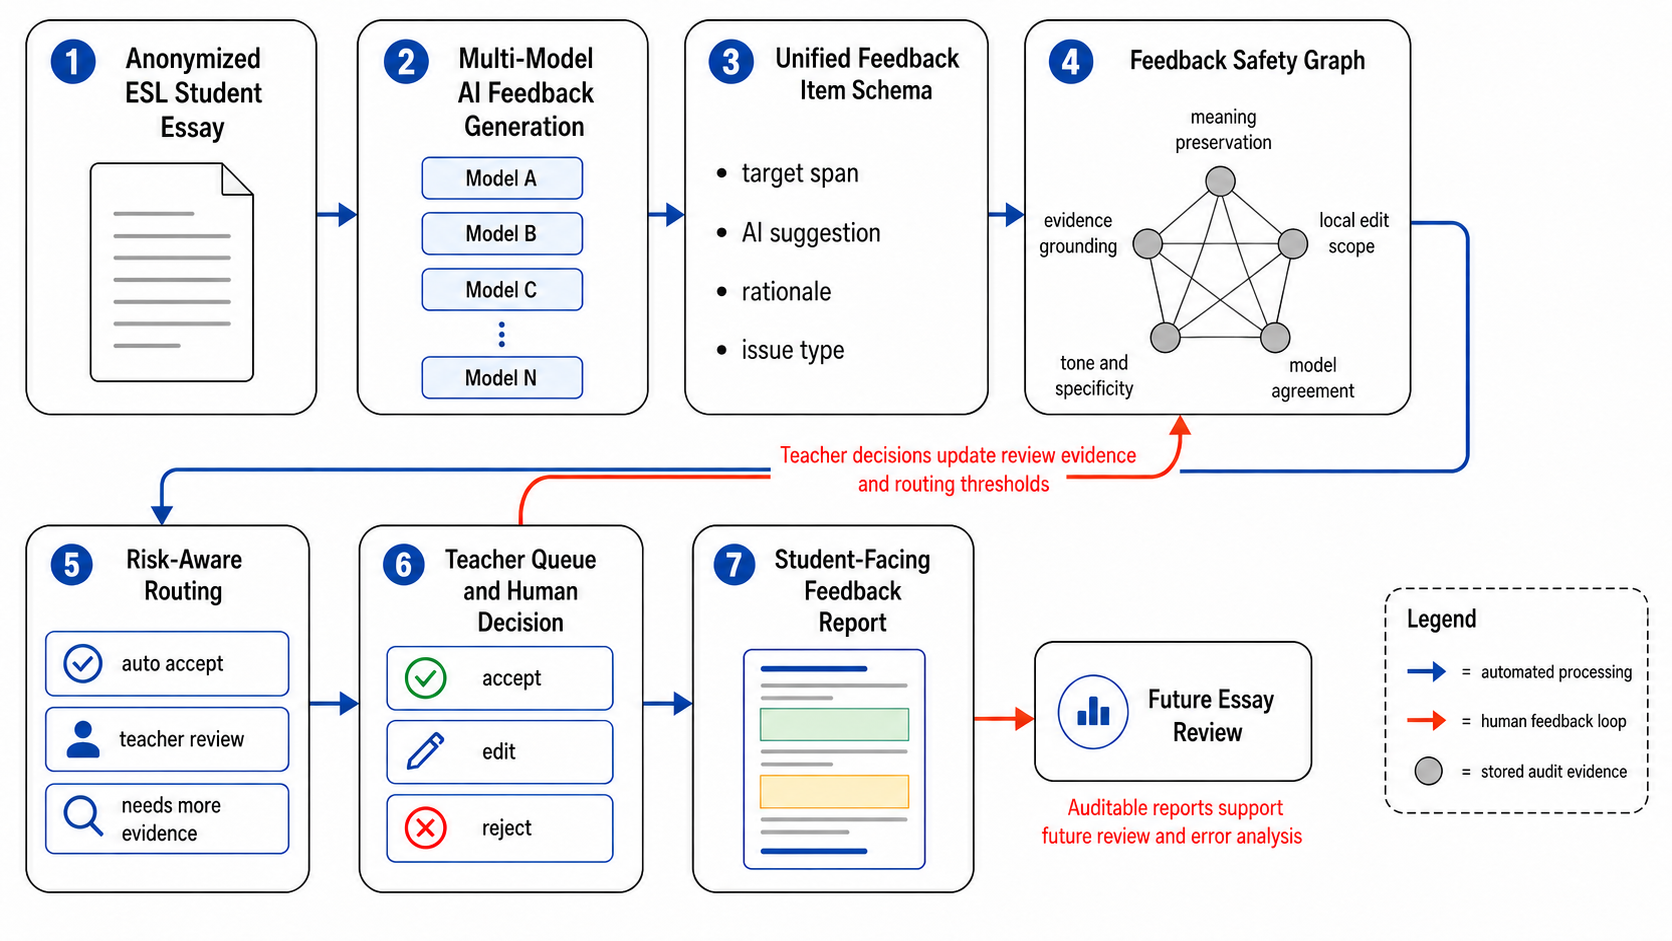
\includegraphics[width=0.94\linewidth]{figures/feedback_safety_routing_cycle.png}
\caption{ConsensusScope workflow for safety routing of AI-generated ESL writing
feedback. Blue arrows denote automated processing from anonymized essays and
multi-model feedback to item-level routing decisions; red arrows denote teacher
feedback loops that update review evidence and future audit analysis.}
\label{fig:routing-cycle}
\end{figure*}

We evaluate this middle layer with stress checks, a public learner-corpus
benchmark over 349,782 generated feedback candidates, and a 30-item two-teacher
diagnostic pilot. The evidence supports a narrow claim: ConsensusScope can
auto-route low-risk feedback while keeping constructed unsafe items in the
review queue. It does not replace teachers or measure classroom learning gains.
The demo contributes a safety-routing formulation, a Feedback Safety Graph
Routing algorithm with pilot-calibrated release policy, a usable
Streamlit/FastAPI review system, and a reproducible evaluation package for
teacher-supervised AI feedback.

\section{Related Work}

\paragraph{Learner writing and GEC.}
GEC benchmarks have provided standardized correction tasks and learner-writing
data, including CoNLL-2014~\cite{ng-etal-2014-conll}, BEA-2019
W\&I+LOCNESS~\cite{bryant-etal-2019-bea}, FCE~\cite{yannakoudakis2011fce}, and
JFLEG~\cite{napoles-etal-2017-jfleg}. Earlier shared tasks and corpora such as
HOO and NUCLE helped establish learner-text correction as a benchmarked NLP
problem~\cite{dale-kilgarriff-2011-helping,dahlmeier-etal-2013-building}.
Phrase-level edit extraction and scorer conventions such as M2 and ERRANT
further standardized how original/corrected pairs are converted into edit
records~\cite{dahlmeier-ng-2012-better,bryant-etal-2017-automatic}. These
datasets primarily evaluate correction quality. ConsensusScope uses their
correction annotations only as offline evidence for a downstream routing
question: whether risky or incorrect feedback candidates remain in a review
queue.

\paragraph{Automated writing feedback.}
Automated writing systems can provide revision support, but classroom use
depends on how learners and teachers interpret the feedback
~\cite{madnani-etal-2018-writing,ranalli2018automated}. ConsensusScope follows
this caution by avoiding a teacher-replacement claim and making AI feedback
inspectable before it becomes student-facing.

\paragraph{LLM reliability and adjudication.}
Multi-output and judge-based methods can help select answers or evaluate
generations~\cite{wang2023selfconsistency,zheng2023judging,liu2023geval}.
However, consensus or judge confidence is not equivalent to educational safety.
Our demo treats model agreement as one observable signal alongside issue type,
evidence status, meaning-change warnings, unsupported-claim cues, tone cues,
and parse errors.

Unlike GEC tools, essay scorers, or generic LLM-as-judge workflows,
ConsensusScope routes each \emph{feedback item} before it reaches a student and
exposes graph evidence behind release or review decisions.

\begin{table*}[t]
\centering
\small
\setlength{\tabcolsep}{4pt}
\begin{tabular}{@{}p{0.18\linewidth}p{0.17\linewidth}p{0.20\linewidth}p{0.35\linewidth}@{}}
\toprule
System type & Main object & Typical output & ConsensusScope distinction \\
\midrule
GEC / revision tools & Sentence edit & Corrected text & Audits whether feedback should be student-facing \\
Essay scoring systems & Whole essay & Score or rubric label & Avoids grading and routes item-level AI feedback \\
LLM-as-judge workflows & Model output & Preference or quality score & Uses graph-backed deploy-time safety signals \\
Feedback dashboards & Review records & Tables or filters & Connects target span, suggestion, risk, route, and teacher action \\
\bottomrule
\end{tabular}
\caption{ConsensusScope is positioned as feedback safety routing rather than
automatic correction, essay scoring, or generic model judging.}
\label{tab:comparison}
\end{table*}


\section{Method}

ConsensusScope implements Feedback Safety Graph Routing (FSGR), an item-level
routing method for deciding whether an AI-generated writing-feedback suggestion
can be shown to a student. The workflow has three input-output modules: given
an anonymized essay $E$ and feedback candidates $\mathcal{C}=\{c_i\}_{i=1}^{n}$,
Module 1 normalizes each candidate, Module 2 builds graph-backed safety
evidence, and Module 3 maps that evidence to a route
$r_i\in\{A,V,E\}$, where $A$ denotes automatic release, $V$ denotes teacher
review, and $E$ denotes a request for more evidence.

\paragraph{Module 1: unified feedback item.}
FSGR first normalizes each raw candidate into a stable schema
$f_i=(d_i,x_i,z_i,u_i,h_i,t_i,a_i)$: essay id, target span, surrounding context,
AI suggestion, rationale, predicted issue type, and optional agreement signal.
This makes live OpenAI-compatible feedback, deterministic benchmark candidates,
and stored audit records enter the same downstream router. The module output is
the comparable feedback item $f_i$.

\paragraph{Module 2: Feedback Safety Graph.}
The router extracts deploy-time signals for parse failure, evidence gaps,
meaning-change cues, unsupported claims, whole-draft rewriting, tone warnings,
teacher-dependent wording, broad target spans, and agreement risk. These signals
activate graph dimensions for local edit, meaning preservation, content
grounding, pedagogical tone, feedback specificity, and model agreement. The
stored path has the form
\textit{target span $\rightarrow$ AI suggestion $\rightarrow$ active safety
dimension $\rightarrow$ route}, so teachers can inspect why an item is released
or queued. The module output is the graph record $G_i$ and its active safety
signals.

\paragraph{Module 3: release policy.}
FSGR computes a bounded risk score and a calibrated review probability,
\[
s_i=\min(1,\sum_k \alpha_k b_{ik}),\quad
p_i=\sigma(\beta_0+\beta^\top x_i),
\]
where $b_i$ is the deploy-time signal vector and $x_i$ combines risk score and
active graph dimensions, following the logistic regression formulation
~\cite{cox1958regression}. High-severity signals and parse/evidence failures
can override the probability. The module output is the final route:
\[
r_i =
\begin{cases}
E, & \phi_i=1,\\
V, & h(b_i)=1 \vee p_i\ge \tau,\\
A, & \text{otherwise}.
\end{cases}
\]
Teacher ratings and public-corpus gold corrections are used only for offline
calibration and evaluation; they are not available when routing a new item.

\section{System Interface}

The demo turns FSGR into a teacher-facing review workflow. In single-essay mode,
a teacher reviews an anonymized ESL draft and inspects item-level routes. In
batch mode, the system prioritizes medium- and high-risk feedback in a teacher
queue before exporting a student-facing report. The FastAPI backend exposes the
same router for programmatic use, returning the route, risk reasons, calibrated
review probability, and graph record.

\begin{figure}[t]
\centering
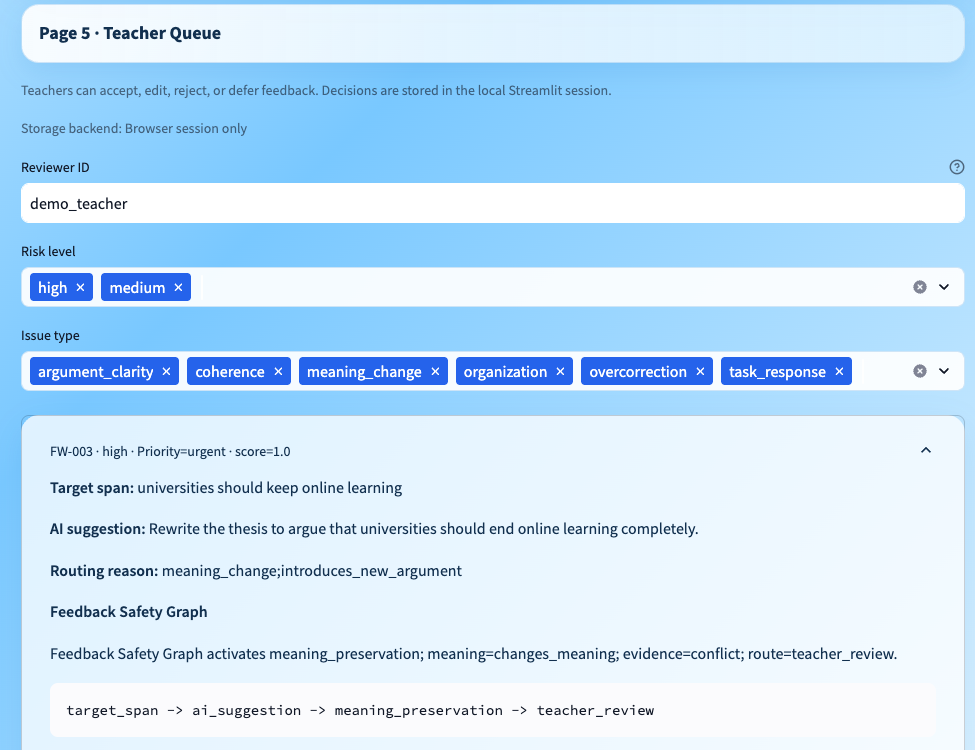
\includegraphics[width=\linewidth]{figures/demo_teacher_queue_cropped.png}
\caption{Teacher Queue in the ConsensusScope demo. The interface filters risky
feedback, displays the target span and AI suggestion, and exposes the Feedback
Safety Graph path before teacher release.}
\label{fig:teacher-queue}
\end{figure}

The main users are English writing teachers, educational NLP developers, and
researchers studying human-in-the-loop feedback. Teachers use the queue to
separate low-risk local edits from suggestions requiring professional judgment.
Developers use the unified records to debug generators, and researchers can
compare routing policies and teacher-aligned diagnostics. The system is useful
even when the underlying feedback generator changes, because the routing layer
only assumes the unified feedback schema.


\section{Evaluation}

We evaluate ConsensusScope as a review-routing layer, not as a feedback
generator, GEC model, or measure of student learning gains. The comparison
question is whether FSGR gives a better safety-efficiency trade-off than simpler
release policies such as review-all or more permissive automatic release. We
measure unsafe-feedback recall in the review queue, auto-release share, and
alignment with teacher-facing diagnostics. We do not run end-to-end comparisons
with commercial AI writing-feedback products or compare GPT/Llama-style feedback
generation quality, because the task is safety routing for feedback suggestions.

\paragraph{Stress checks and public benchmark.}
The packaged demo contains 31 stress and expected-route cases covering thesis
reversal, unsupported factual claims, whole-essay rewriting, harsh tone, low
agreement, and parse failures; the router matches the expected route labels. For
a larger offline benchmark, we use public learner-correction corpora:
JFLEG~\cite{napoles-etal-2017-jfleg}, CoNLL-2014~\cite{ng-etal-2014-conll},
FCE~\cite{yannakoudakis2011fce}, and W\&I+LOCNESS~\cite{bryant-etal-2019-bea}.
We use edit-distance alignment~\cite{levenshtein1966binary}, following
edit-centric GEC evaluation
~\cite{dahlmeier-ng-2012-better,bryant-etal-2017-automatic}. Each public gold
edit yields one correct feedback candidate and one or two constructed risk
distractors. Thus the 349,782 candidates are derived from 117,401 public gold
edits plus 232,381 constructed risk distractors, not newly collected student
records or uncontrolled LLM generations.

\begin{table}[t]
\centering
\scriptsize
\resizebox{\columnwidth}{!}{%
\begin{tabular}{lrrrrrrr}
\toprule
Source & Records & Gold edits & Correct cand. & Risk dist. & Candidates & Auto & Review \\
\midrule
JFLEG & 1,501 & 3,938 & 3,938 & 7,649 & 11,587 & 0.320 & 0.680 \\
CoNLL-2014 & 2,624 & 5,110 & 5,110 & 10,016 & 15,126 & 0.324 & 0.676 \\
FCE & 33,236 & 45,969 & 45,969 & 90,965 & 136,934 & 0.329 & 0.671 \\
W\&I+LOCNESS & 38,692 & 62,384 & 62,384 & 123,751 & 186,135 & 0.329 & 0.671 \\
\midrule
Total & 76,053 & 117,401 & 117,401 & 232,381 & 349,782 & 0.328 & 0.672 \\
\bottomrule
\end{tabular}
}
\caption{Public learner-corpus routing benchmark. Candidate counts are derived
from public gold edits: each edit contributes one correct candidate and one or
two constructed risk distractors.}
\label{tab:public}
\end{table}

\paragraph{Teacher diagnostics and routing utility.}
A blind two-teacher pilot over 30 anonymized AI feedback items checks whether
routes align with human judgments on correctness, meaning preservation, student
readiness, usefulness, clarity, and direct-release suitability. The pilot is a
diagnostic study, not a classroom trial: the router obtains 1.000 recall for
teacher-marked review-needed and unsafe items, 0.857 auto-accept precision
against teacher-safe items, and 0.694 within-one-point teacher agreement.
Table~\ref{tab:policy} compares FSGR with two policy baselines: review-all and
a more permissive low/medium-risk release policy. The default policy
auto-routes 32.9\% of candidates while preserving all constructed incorrect or
unsafe candidates in the review queue.

\begin{table}[t]
\centering
\scriptsize
\setlength{\tabcolsep}{2pt}
\begin{tabular}{p{0.39\linewidth}rrrr}
\toprule
Policy & Auto & Acc. & Review & Err. rev. \\
\midrule
Accept low; review med/high & 0.329 & 1.000 & 0.671 & 1.000 \\
Accept low/med; review high & 0.336 & 1.000 & 0.664 & 1.000 \\
Review all & 0.000 & -- & 1.000 & 1.000 \\
\bottomrule
\end{tabular}
\caption{Pooled review-routing utility. Err. rev. is the share of observed
incorrect or unsafe candidates routed to human review.}
\label{tab:policy}
\end{table}

The evaluation supports a conservative deployment claim: ConsensusScope does
not make AI feedback automatically correct, but it makes feedback release
observable and keeps high-risk suggestions under teacher control.

\section{Availability and Reproducibility}

The repository, live demo, video, and API documentation are available at
\url{https://github.com/yyting2006-ai/ConsensusScope},
\url{https://demo.consensusscope.cn/},
\url{https://youtu.be/vp4Kj48bv8Q}, and
\url{https://api.consensusscope.cn/docs}. The repository includes startup
instructions and \texttt{scripts/run\_public\_gec\_benchmark.py}; raw corpora
and per-item derived outputs are not committed.

\section{Ethics and Limitations}

ConsensusScope is a teacher-support tool, not an automatic essay scorer or
teacher replacement. Users should upload only anonymized student writing. The
benchmark validates graph-backed routing with public correction labels and
constructed distractors; it does not measure learning gains, time-on-task, or
real LLM feedback quality. The teacher pilot is diagnostic, not a classroom
study.

\section{Conclusion}

ConsensusScope demonstrates safety routing for generative AI English essay
feedback: it converts feedback items into graph-backed release decisions so
teachers can reduce review burden without giving up control over what students
receive.

\begingroup
\small
\bibliography{references}
\endgroup

\appendix

\section{Supplementary Implementation Details}

This appendix provides compact implementation artifacts for reproducing the
routing behavior described in the main paper. The appendix is not used to add
new experimental claims; it documents the router, exported fields, and pilot
case patterns.

\paragraph{Router pseudocode.}
\begin{center}
\setlength{\fboxsep}{5pt}
\fbox{\begin{minipage}{0.93\linewidth}
\scriptsize
\textbf{Algorithm A.1: Feedback Safety Graph Router}\\
\textbf{Input:} normalized item $f_i$, local context $z_i$, optional rationale
$h_i$, agreement signal $a_i$\\
\textbf{Output:} route $r_i$, review probability $p_i$, risk score $s_i$, graph
$G_i$
\begin{enumerate}
\setlength{\itemsep}{0pt}
\setlength{\parsep}{0pt}
\item Extract deploy-time signals $b_i$ for parse failure, evidence conflict,
meaning-change cues, unsupported claims, tone warnings, broad target spans, and
agreement risk.
\item Map $b_i$ to graph dimensions: local edit, meaning preservation, content
grounding, pedagogical tone, feedback specificity, and model agreement.
\item Construct $G_i$ with target-span, suggestion, evidence, dimension, and
route nodes.
\item Compute $s_i=\min(1,\sum_k\alpha_k b_{ik})$.
\item Build $x_i=[s_i;\mathrm{active\ dimensions}]$ and compute
$p_i=\sigma(\beta_0+\beta^\top x_i)$.
\item If parse or grounding failure is active, set $r_i=E$.
\item Else if a high-severity signal is active or $p_i\ge\tau$, set $r_i=V$.
\item Else set $r_i=A$.
\item Return $r_i$, $p_i$, $s_i$, risk reasons, graph path, and JSON records.
\end{enumerate}
\end{minipage}}
\end{center}

The actions $E$, $V$, and $A$ denote evidence request, teacher review, and
automatic release. High-severity graph signals can override the calibrated
probability so that clearly unsafe feedback remains in the teacher queue.

\paragraph{Calibration artifact.}
\begin{table}[h]
\centering
\scriptsize
\begin{tabular}{lr}
\toprule
Feature & Weight \\
\midrule
Intercept & -0.582 \\
Risk score & 0.861 \\
Local-edit signal & -0.467 \\
Meaning-risk signal & 1.138 \\
Grounding-risk signal & 0.653 \\
Specificity-risk signal & -0.047 \\
Agreement-risk signal & 0.000 \\
Evidence-gap signal & 0.000 \\
\bottomrule
\end{tabular}
\caption{Pilot-calibrated logistic release weights. The cutoff is
$\tau=0.300$ and is stored in \texttt{routing\_calibration.json}.}
\label{tab:appendix-calibration}
\end{table}

\paragraph{Exported audit fields.}
\begin{table}[h]
\centering
\scriptsize
\begin{tabular}{ll}
\toprule
Output field & Stored value \\
\midrule
\texttt{risk\_level} & Risk label \\
\texttt{recommended\_action} & Release route \\
\texttt{review\_probability} & Calibrated probability \\
\texttt{safety\_graph\_path} & Explanation path \\
\texttt{safety\_graph\_nodes} & JSON node records \\
\texttt{safety\_graph\_edges} & JSON edge records \\
\texttt{teacher\_action} & Accept/edit/reject/defer \\
\bottomrule
\end{tabular}
\caption{Core fields exported for each routed feedback item.}
\label{tab:appendix-fields}
\end{table}

\paragraph{Representative routed cases.}
\begin{table}[h]
\centering
\scriptsize
\resizebox{\columnwidth}{!}{%
\begin{tabular}{llll}
\toprule
Case & Pattern & Route & Diagnostic use \\
\midrule
FB-002 & Local phrase edit & Auto & Teachers rate safe \\
FB-003 & Thesis reversal & Review & Blocks meaning change \\
FB-005 & Wrong modal edit & Review & Finds unsafe local edit \\
FB-008 & Unsupported claim & Review & Blocks evidence gap \\
\bottomrule
\end{tabular}
}
\caption{Representative pilot cases. Teacher ratings are offline diagnostics,
not deploy-time labels.}
\label{tab:appendix-cases}
\end{table}

\paragraph{Reproducibility checklist.}
The released package includes the Streamlit entry point, FastAPI router,
sample ESL feedback items, stress cases, public-benchmark construction script,
routing calibration file, and report-export templates. To reproduce the main
benchmark, users run \texttt{scripts/run\_public\_gec\_benchmark.py} after
placing the required public learner corpora outside the repository. The
generated per-item benchmark outputs are intentionally not committed because of
size and redistribution constraints.

\paragraph{Input schemas.}
ConsensusScope keeps generation, routing, and teacher review separable by using
explicit CSV/JSON schemas. The essay table stores anonymized writing context;
the feedback table stores model suggestions; the routing table stores deploy-time
signals and graph records. The router does not require teacher labels when a new
feedback item is processed.

\begin{table}[h]
\centering
\scriptsize
\resizebox{\columnwidth}{!}{%
\begin{tabular}{ll}
\toprule
Schema & Required fields \\
\midrule
Essay & id, prompt, genre, level, anonymized text, word count, draft stage \\
Feedback item & id, essay id, target span, context, suggestion, rationale, source, issue type \\
Routing result & risk level, action, reasons, review probability, graph path, nodes, edges \\
\bottomrule
\end{tabular}
}
\caption{Input and output schemas used by the demo and benchmark scripts.}
\label{tab:appendix-schema}
\end{table}

\paragraph{Deploy-time signals.}
The router uses only signals observable before a teacher makes a decision. This
separation prevents offline labels from leaking into deployment. Gold edits and
teacher ratings are used after routing to evaluate whether the queue captured
unsafe or review-needed items.

\begin{center}
\centering
\scriptsize
\begin{tabular}{p{0.30\linewidth}p{0.55\linewidth}}
\toprule
Signal group & Examples \\
\midrule
Meaning preservation & thesis reversal, changed stance, overgeneralization \\
Content grounding & unsupported evidence, invented study, exam-score claim \\
Local edit scope & article/preposition edit, narrow vocabulary substitution \\
Pedagogical tone & harsh wording, student-level mismatch, vague advice \\
System status & parse failure, missing context, low agreement \\
\bottomrule
\end{tabular}
\par\smallskip
\footnotesize\textbf{Table 8:} Deploy-time signal groups mapped to Feedback
Safety Graph dimensions.
\end{center}

\begin{center}
\scriptsize
\begin{tabular}{p{0.30\linewidth}p{0.55\linewidth}}
\toprule
Route & Operational meaning \\
\midrule
\texttt{auto\_accept} & The item is a narrow local edit with no active
meaning-change, grounding, or tone warning. \\
\texttt{teacher\_review} & The item may be useful, but a teacher should inspect
the span, rationale, or graph path before release. \\
\texttt{needs\_more\_}\newline\texttt{evidence} & The item cannot be grounded in the available
essay context or failed parsing, so it is held back. \\
\bottomrule
\end{tabular}
\par\smallskip
\footnotesize\textbf{Table 9:} Release semantics exposed to teachers and
stored in the audit log.
\end{center}

\paragraph{Minimal audit record.}
Each routed item exports the same compact record for later review:
\begin{center}
\fbox{\begin{minipage}{0.92\columnwidth}
\scriptsize
\texttt{\{}\\
\texttt{\ \ "feedback\_item\_id": "FB-008",}\\
\texttt{\ \ "route": "teacher\_review",}\\
\texttt{\ \ "review\_probability": 0.84,}\\
\texttt{\ \ "risk\_reasons": ["unsupported\_claim"],}\\
\texttt{\ \ "graph\_path": ["content\_grounding", "review"]}\\
\texttt{\}}
\end{minipage}}
\end{center}

\paragraph{Teacher workflow.}
In a live review session, a teacher first filters the queue by risk level or
issue type, opens an item, checks the target span and suggestion, and then
inspects the graph path. The teacher can accept, edit, reject, or defer the
item. Only accepted or edited items are exported into the student-facing report.
The audit log keeps the route, graph path, risk reasons, and teacher action so
that later error analysis can identify which feedback patterns repeatedly need
human review.

\paragraph{Comparison boundary.}
The current benchmark is intentionally a routing benchmark. It compares release
policies over the same feedback candidates rather than comparing feedback
generators. This is important for deployment: a school may replace the LLM or
prompt, but the review-routing layer should still expose whether a concrete
suggestion is safe to release. End-to-end learning gains, teacher time savings,
and commercial-system comparisons are left for future classroom studies.

\paragraph{Benchmark accounting.}
The public-corpus benchmark converts learner edits into item-level feedback
events so that release policies can be tested without collecting new student
records. The same router is then run over all constructed items.

\begin{center}
\scriptsize
\begin{tabular}{lr}
\toprule
Benchmark item type & Count \\
\midrule
Gold edit feedback items & 117,401 \\
Constructed risk distractors & 232,381 \\
Total routed candidates & 349,782 \\
\bottomrule
\end{tabular}
\par\smallskip
\footnotesize\textbf{Table 10:} Public benchmark accounting used for the
routing evaluation.
\end{center}

\paragraph{Teacher pilot form.}
The teacher study uses a blind item-level rating form. Teachers see the
anonymized essay context, target span, AI suggestion, and rationale, but not the
system route, graph score, model identity, or agreement signal.

\begin{center}
\scriptsize
\begin{tabular}{p{0.38\linewidth}p{0.47\linewidth}}
\toprule
Rating dimension & Question focus \\
\midrule
Correctness & Is the feedback linguistically or pedagogically correct? \\
Meaning preservation & Does it keep the student's intended meaning? \\
Student readiness & Can it be shown directly to a learner? \\
Usefulness & Would it help revision? \\
Clarity & Is the suggestion understandable? \\
Direct-release suitability & Can it bypass teacher editing? \\
\bottomrule
\end{tabular}
\par\smallskip
\footnotesize\textbf{Table 11:} Blind teacher-rating dimensions used only for
offline diagnosis and calibration.
\end{center}

\paragraph{Reproduction steps.}
The submission package separates sensitive data, generated benchmark outputs,
and source code. Reviewers can inspect the demo with sample data and reproduce
the routing tables after placing public learner corpora in a local data folder.

\begin{center}
\fbox{\begin{minipage}{0.92\columnwidth}
\scriptsize
1. Install package requirements and start the Streamlit/FastAPI demo.\\
2. Place public learner-corpus files outside the repository.\\
3. Run the public GEC benchmark construction script.\\
4. Run the routing evaluation and regenerate report tables.\\
5. Export audit logs for manual inspection.
\end{minipage}}
\end{center}

\end{document}
